\documentclass[a4paper]{article}
\usepackage[letterpaper,top=2cm,bottom=2cm,left=3cm,right=3cm,marginparwidth=1.75cm]{geometry}
\usepackage[colorlinks=true, allcolors=blue]{hyperref}

\usepackage{wrapfig}
\usepackage{amsthm}
\usepackage{hyperref}
\usepackage{graphicx}
\usepackage{amsfonts}

\title{CUDA HW2}
\author{Patryk Drozd}
\begin{document}
\date{}
\maketitle

\section{Overview}

	The data used for these plots was obained whe cuda01 was in use by other
	users and myself so I imagine that the runtimes might be a bit inconsistent.
	The code is stored in "/home/users/mschpc/2024/drozdp/my\_shtuff/homeworks/hw2"
	on cuda01.

	The code is structured as follows. At the top direcotry the "float" and "double" 
	directories hold the main parts of the code with each being a copy of the other
	with the exception that one stores memory in doubles and one in floats. 
	"comarison\_plots" hold some plots and scpits for comparing the float and double
	codes with eachother. "report" holds this file and the pdf version. 

	Within each of "double" and "float" verisons both hold cpu and gpu files
	with a "writeup" directory which hold runtime data and plots. The ".c" and ".cu"
	files are the main bits of code while the ".sh" files hold a bash srcipt to 
	execute the "c" and "cu" files. The ".py" files are for producing the plots.

\section{Task1}

    Task 1 is done in files task1.c and task1\_funcs.c and is later copied in 
	task2.cu for easier comparison. 

\section{Task2}
		
	The gpu implementaion is written in task2.cu and task2\_funcs.cu. 
	The precision is in line with the difference being less than 1w-4.

	The relevant timings are obained as the code executes and it prints them out
	on the go. Below is an example of a sample size of code run and some timings.

	\begin{verbatim}
		
	\end{verbatim}

	
	Plots below show speedups with respect to block size in both directions as 
	the code is implemented in a 2d way.
		
	\begin{figure}[h!]
		\centering
		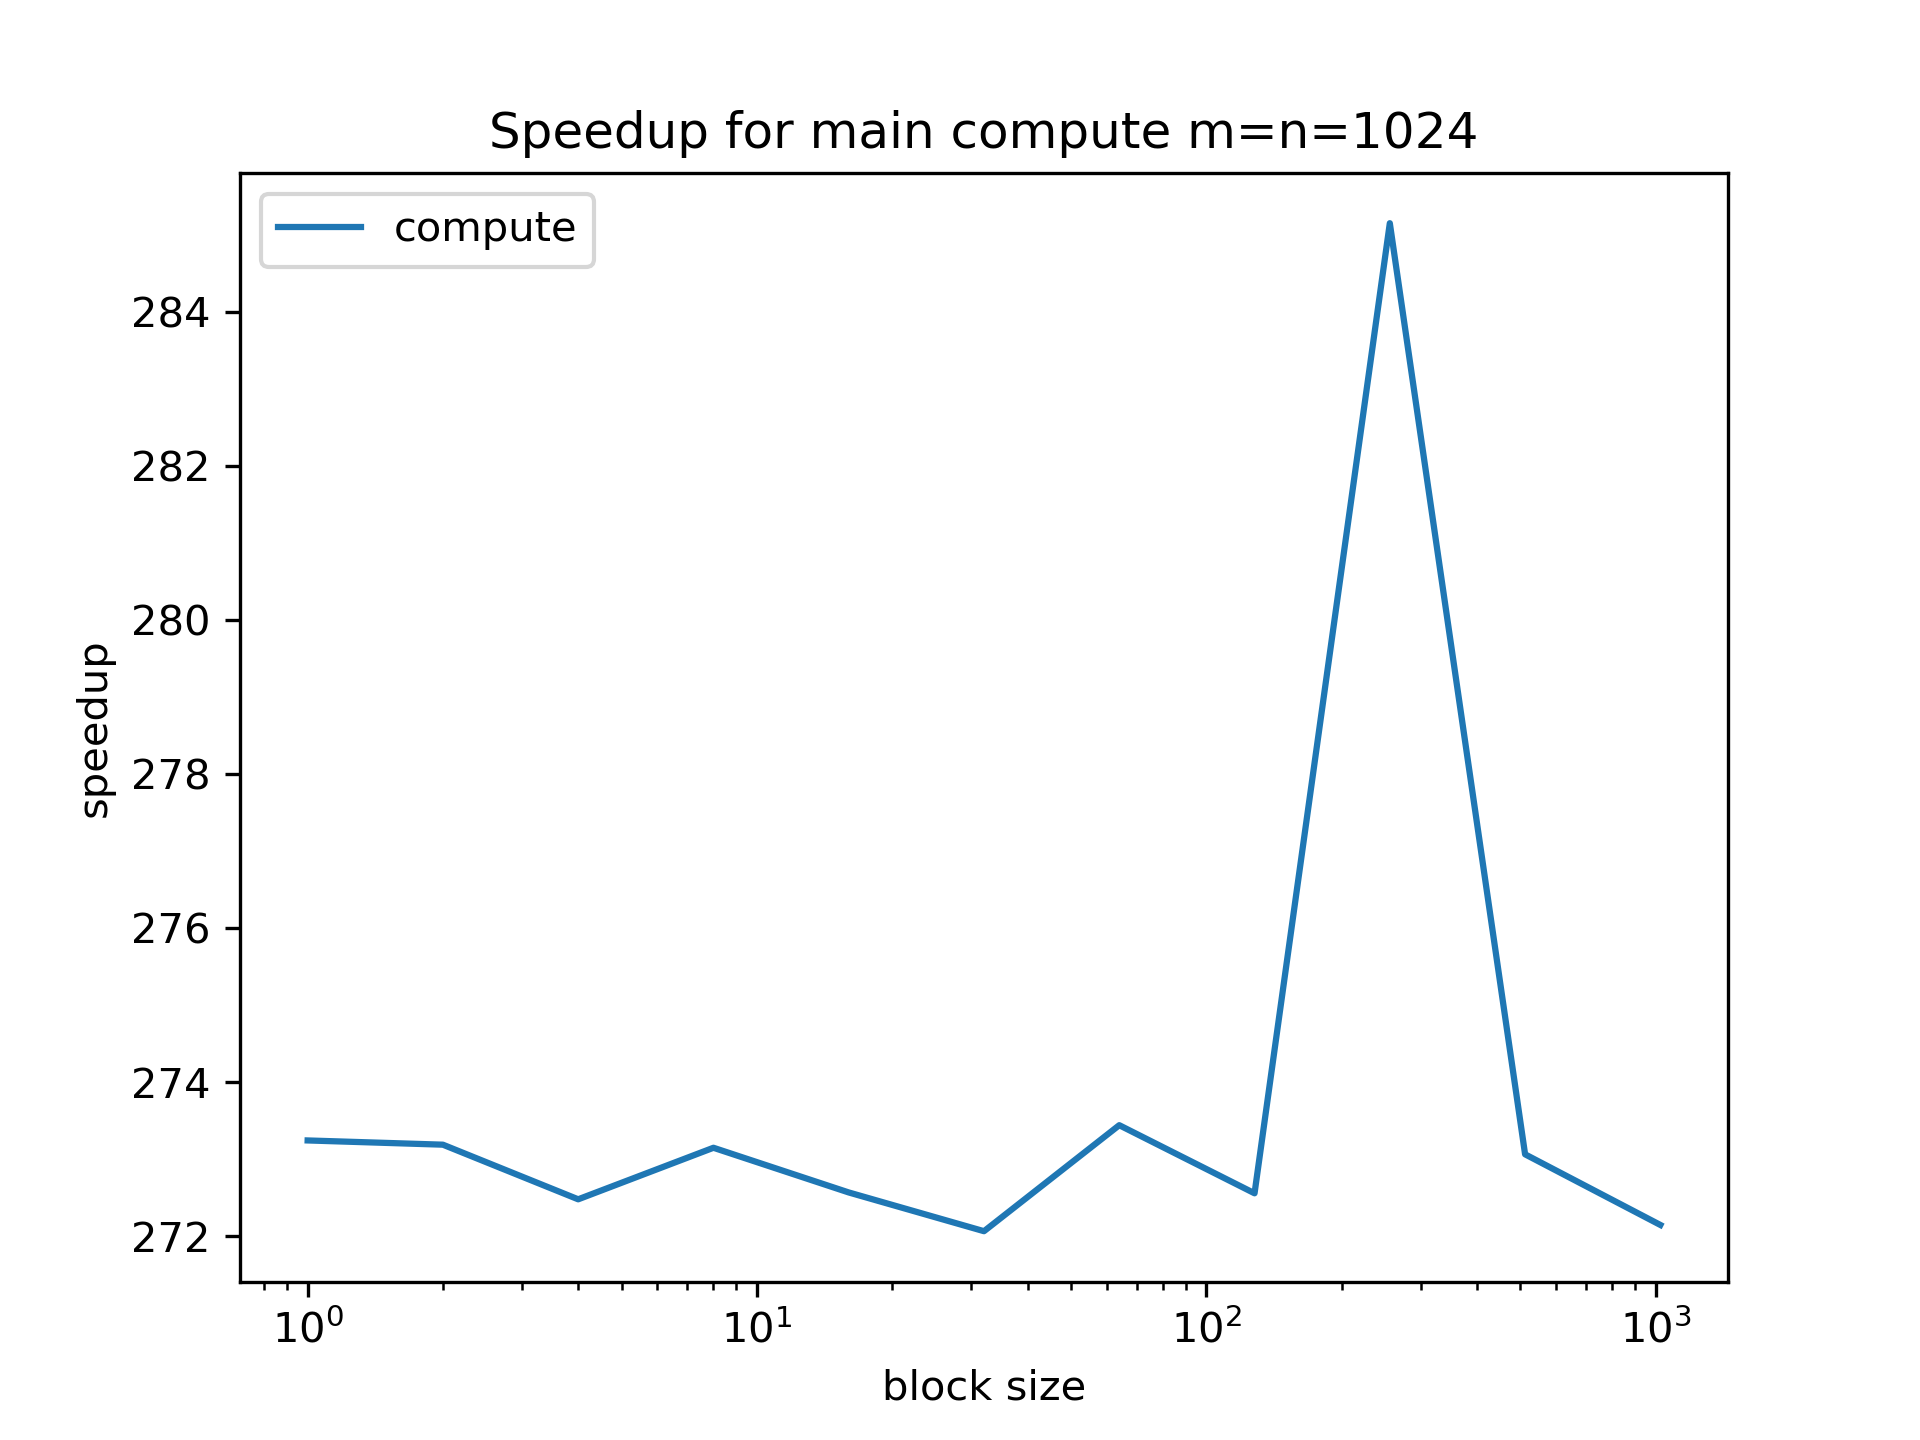
\includegraphics[width=.5\linewidth]{../float/writeup/compute_plot_m1024.png}
		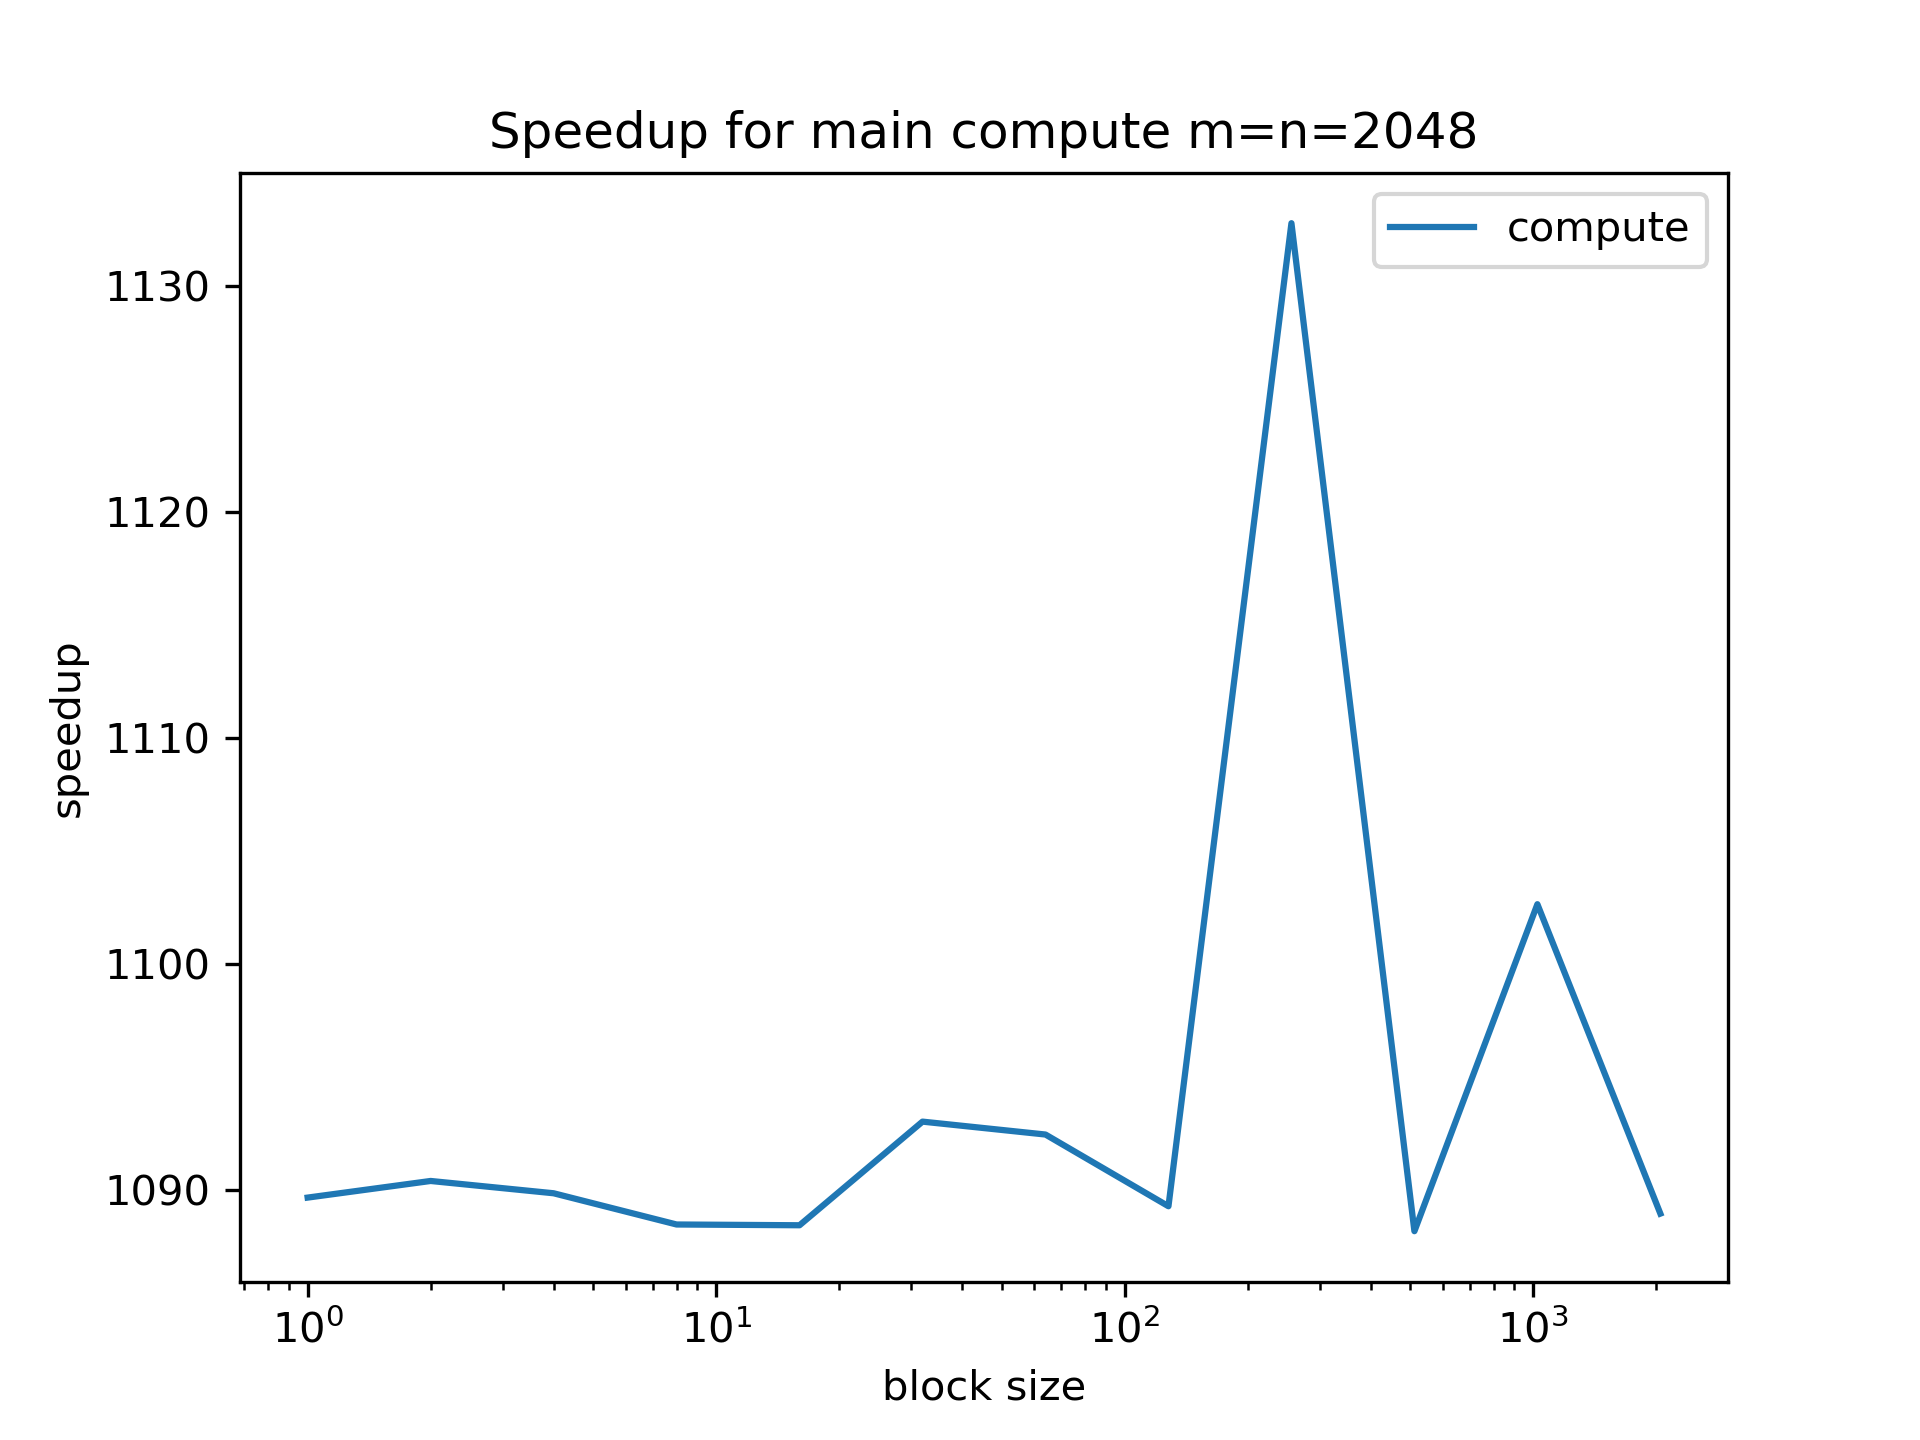
\includegraphics[width=.5\linewidth]{../float/writeup/compute_plot_m2048.png}
		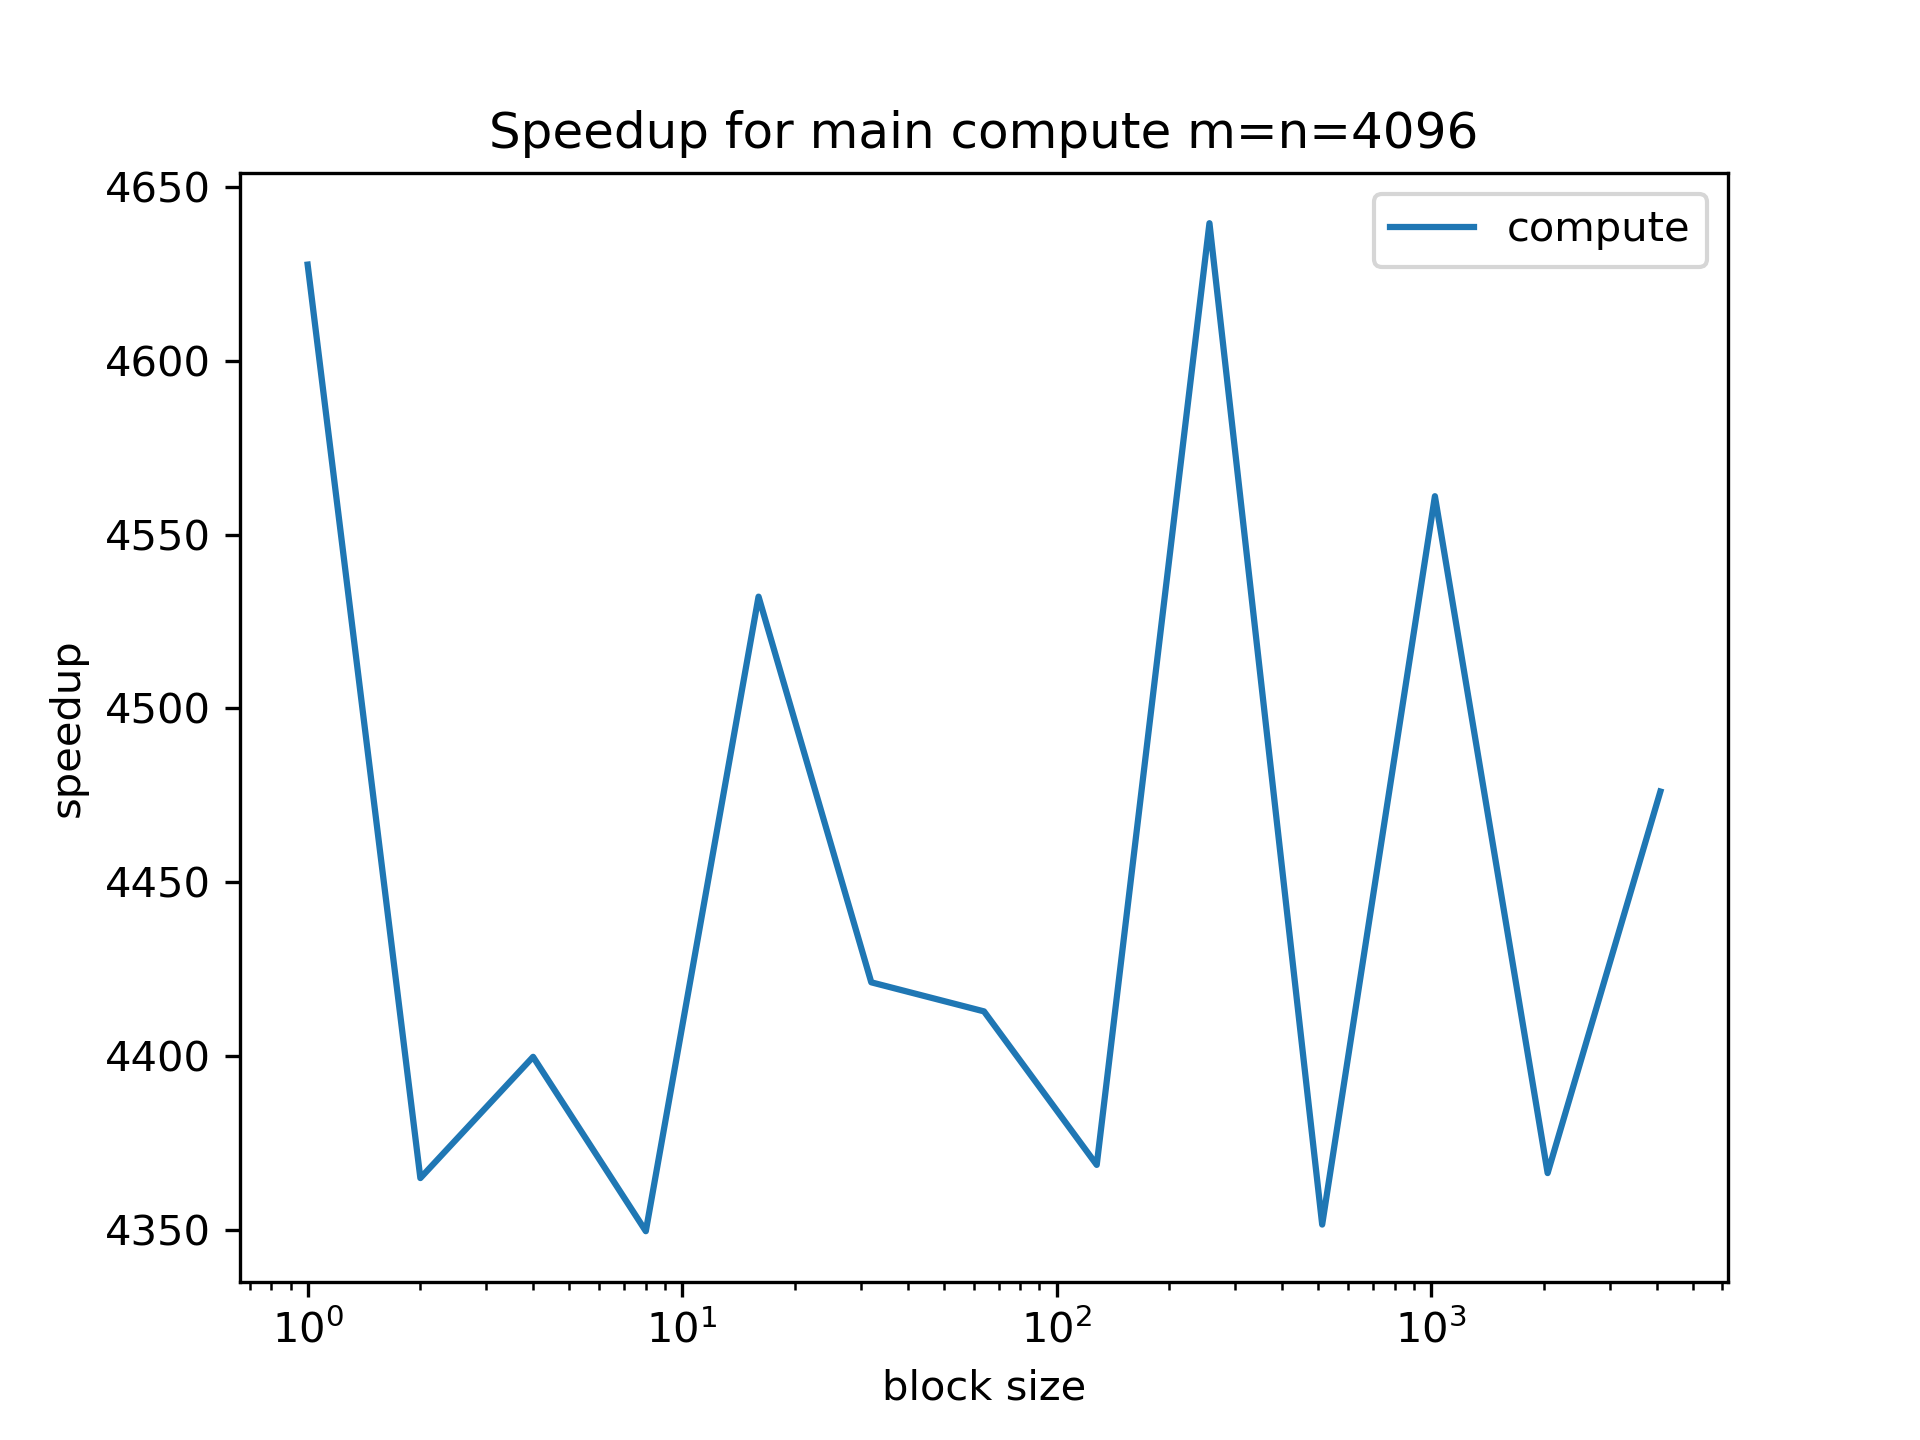
\includegraphics[width=.5\linewidth]{../float/writeup/compute_plot_m4096.png}
		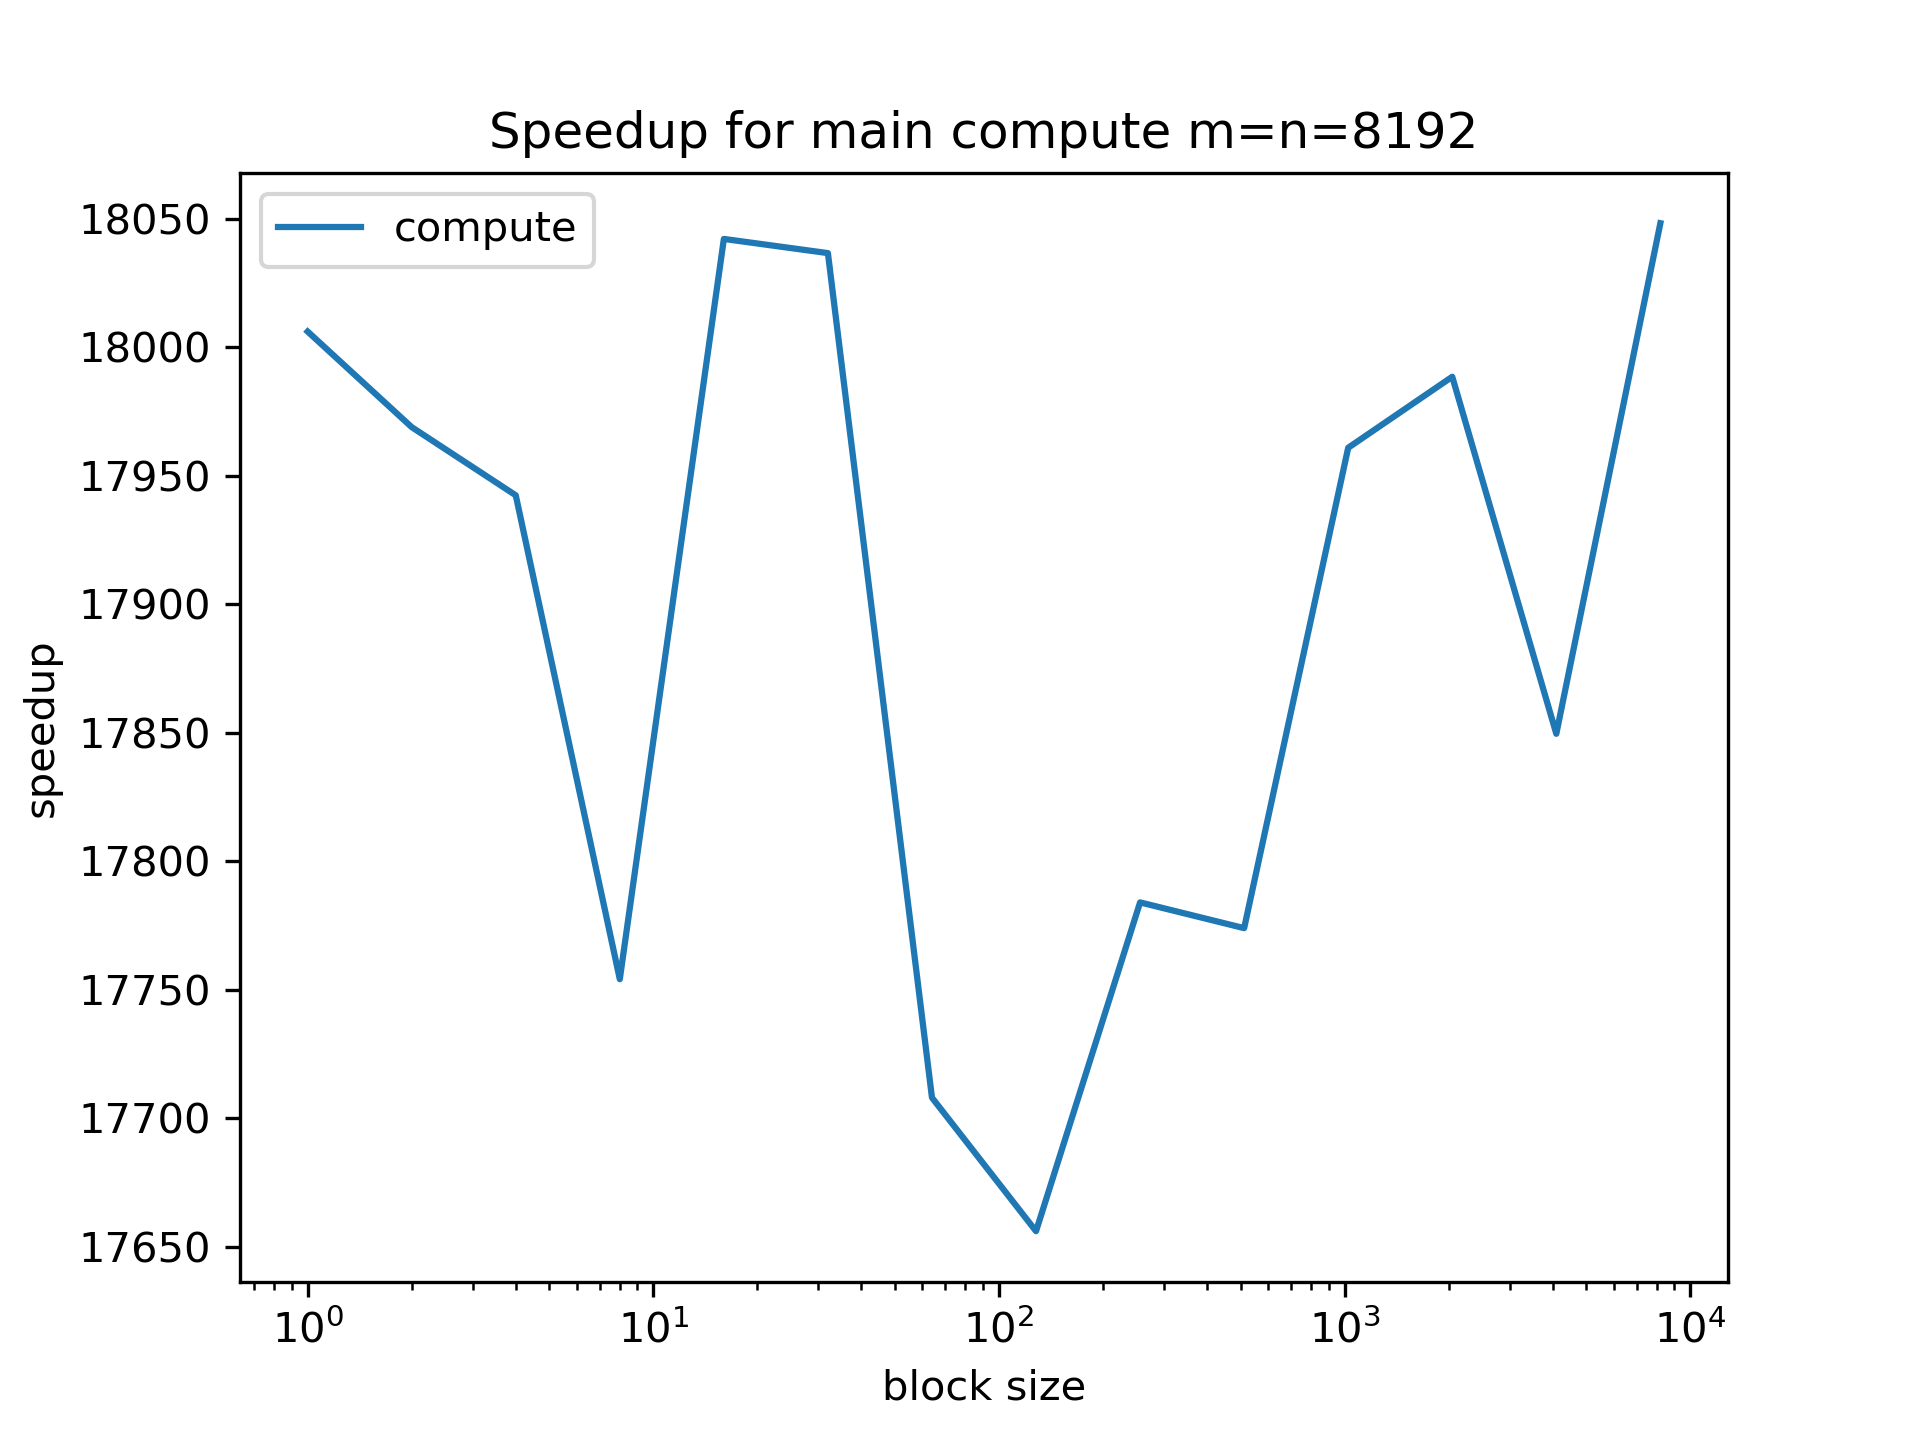
\includegraphics[width=.5\linewidth]{../float/writeup/compute_plot_m8192.png}
		%\label{fig:1}
	\end{figure}


\section{Task3}

	In the figure below I plot the speedup against blocksize for the
	caclulation of the average temperature  compared to using my reduction
	code from homework 1. I

	\begin{figure}[h!]
		\centering
		\includegraphics[width=.5\linewidth]{../float/writeup/reduce_plot_m.1024png}
		\includegraphics[width=.5\linewidth]{../float/writeup/reduce_plot_m.2048png}
		\includegraphics[width=.5\linewidth]{../float/writeup/reduce_plot_m.4096png}
		\includegraphics[width=.5\linewidth]{../float/writeup/reduce_plot_m.8192png}
		%\label{fig:1}
	\end{figure}

\section{Task4}
	
	For this task involving converting the cuda code into double precision I wasnt able
	to completely convert the main iteration loop as surface memory which I was using 
	to store my matrices cant hold double precision numbers easily. Instead I chose to 
	only change the main computation in double precision while storing the results in 
	floating point precision by downcasting the results into floats. Replacing the floats
	with doubles in every other bit of code otherwise worked without much thought.


	\begin{figure}[h!]
		\centering
		\includegraphics[width=.5\linewidth]{../comparison_plots/reduce_plot_m.1024png}
		\includegraphics[width=.5\linewidth]{../comparison_plots/reduce_plot_m.2048png}
		\includegraphics[width=.5\linewidth]{../comparison_plots/reduce_plot_m.4096png}
		\includegraphics[width=.5\linewidth]{../comparison_plots/reduce_plot_m.8192png}
		%\label{fig:1}
	\end{figure}


\bibliographystyle{plain}
\bibliography{refs}

\end{document}

